Ziel des Praktikums war es, eine themenspezifische Suchmaschine zu implementieren, die Wissenschaftliche Publikationen aus dem Fachgebiet der Digital Text Forensics indexieren und durchsuchen kann. 
In der Digital Text Forensics werden Methoden und Verfahren zur Identifikation von Authoren, Erkennung von Plagiaten und Profilerstellung von Authoren untersucht und bereitgestellt. 
Die Publikationen lagen hauptsächlich im PDF-Format und in englischer Sprache vor, weshalb Dokumente in anderen Formaten und Sprachen nicht berücksichtigt wurden. 
Im Verlauf der Vorverarbeitung wurden die Dokumente in ein einheitliches Format und eine einheitliche Zeichenkodierung überführt. 
Um einzelne Bestandteile bzw. Felder eines Dokuments, wie z.B. Titel oder Fließtext, getrennt betrachten zu können, wurde XML als Format gewählt, in das alle Dokument konvertiert und zur Indexierung genutzt werden. 
Die Erkennung und Extraktion einzelner Bestandteile eines Dokuments war dabei eine wesentliche Aufgabe, da Titel der Publikationen als Suchresultat angezeigt werden sollen, diese aber kaum als Meta-Informationen in den PDF-Dokumenten vorhanden waren. 
Das Vorkommen von Wörtern der Suchanfrage in bestimmten Feldern kann somit beim Ranking berücksichtigt werden: Wenn Wörter der Suchanfrage im Titel eines Dokuments vorkommen, wird es als relevanter bewertet, als wenn sie im Fließtext vorkommen. 
Weitere Parameter, die in die Gewichtung der Relevanz eines Dokuments eingehen sind Logdaten, z.B. wie oft ein Dokument für eine Suchanfrage geklickt wurde, sowie die Zeitdauer, die Nutzer auf einem Dokument verbracht haben.
Die Aufzeichnung dieser Daten wurden in einer Datenbank im Backend implementiert, welche auch genutzt wurde, um die Autovervollständigung von Suchanfragen zu ermöglichen. 
Weiterhin geht in die Gewichtung eines Dokuments die Anzahl der Erwähnungen des Dokuments in anderen Publikationen mit ein. 
Zur Ermittlung dieses Kennwertes wurde ein Pearl-Skript geschrieben, sodass dieser Wert bei Erweiterung des Indexes durch neue Dokumente, aktualisiert werden kann. 
Oben genannte Komponenten der Suchmaschine wurden unter Verwendung verschiedener Programmbilbiotheken implementiert, darunter Apache PDFBox, Tika und Docear bei der Vorverarbeitung, Apache Lucene für Indexierung und Suche und das Spring Framework für Backend und Frontend. 
Das Frontend dient als Interface für Suchanfragen eines Nutzers und zur Präsentation der Suchergebnisse, geordnet nach Relevanz und mit einem kurzen Textausschnitt (Snippet) für jedes Suchergebnis. 
In den folgenden Kapiteln wird auf die einzelnen Komponenten der Suchmaschine detailliert eingegangen. 

%% Hier schreibt man dann was. Und so \comment{kommentiert ihr Sachen.}. Offenbar sieht das nicht so schön aus.


%% \begin{figure}[ht]
%%   \subfloat[Pyramidenzelle \label{fig:pyramid_cell}]{%
%%     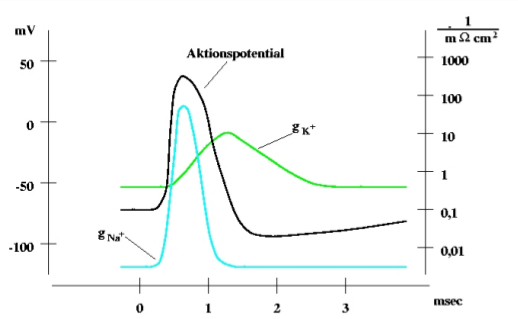
\includegraphics[width=0.4\linewidth]{aktionspotential}
%%   }
%%   \hfill
%%   \subfloat[Neocortex \label{fig:neocortex}]{%
%%     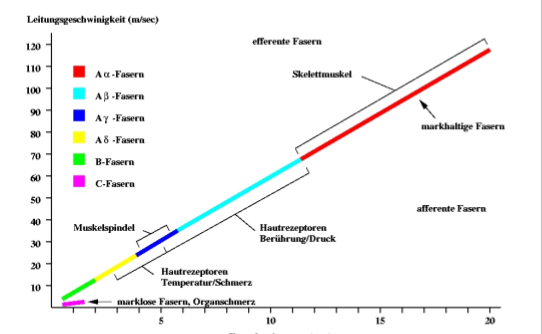
\includegraphics[width=0.5\textwidth]{leitungsgeschwindigkeit}
%%   }
%%   \caption[Aktionspotential und Leitungsgeschwindikeit]{Links:
%%     AP. Rechts: Leitungsgeschwindikeit von verschiedenen Fasern.}
%% \label{fig:ap_leitung}
%% \end{figure}



%%% Local Variables:
%%% mode: latex
%%% TeX-master: "../arbeit"
%%% End:
